\documentclass{article}
\usepackage[utf8]{inputenc}
\usepackage{graphicx}
\usepackage{amssymb}
\usepackage{amsmath}
\title{Assignment 1}
\author{Kotikalapudi Karthik CS21BTECH11030}
\date{29th March 2022}

\begin{document}

\maketitle

\section*{ICSE 2018 Question 9 (c)}
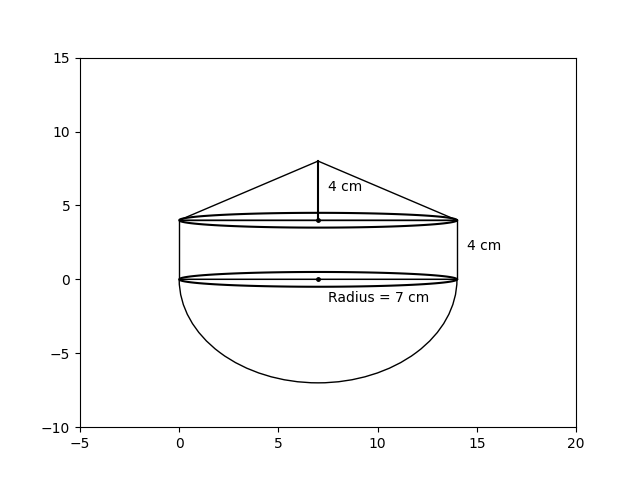
\includegraphics[width=\columnwidth]{question9c.png}
\textbf{Solution :}\\
Here, radius of cone = radius of cylinder = radius of hemisphere = $7cm$\\
Height of cone = Height of cylinder = $4cm$
\begin{align}
    \text{Volume of the figure} &= \text{Vol. of cone + Vol. of cylinder + Vol. of hemisphere}
    \\
    \text{Volume of cone} &= \frac{1}{3} \times \pi \times r^2 \times h = \frac{1}{3} \times \pi \times 49 \times 4 = \frac{196}{3} \times \pi
    \\
    \text{Volume of cylinder} &= \pi \times r^2 \times h = \pi \times 49 \times 4 = 196 \times \pi
    \\
    \text{Volume of hemisphere} &= \frac{2}{3} \times \pi \times r^3 = \frac{2}{3} \times \pi \times 49 \times 4 = \frac{392}{3} \times \pi
\end{align}
$\therefore$From the above equations,\\
Volume of the figure = $\frac{196}{3} \times \pi + 196 \times \pi + \frac{392}{3} \times \pi$\\
$\implies$Volume of the figure = $490 \times \pi \approx 1539.38cm^3$
\end{document}
